\chapter{Tests effectués}

Nous n'avons pas effectué de test sur les fonctions fournies par
le client et les fonctions \textbf{OpenCV} que nous avons utilisé
pour afficher les annotations.

Il est pour nous compliqué de faire des tests sur l'exactitude de
notre affichage. Nous sommes donc concentrés sur des tests
fonctionnels.

\section{Tests sur l'utilisation du Json}

Tous les réglages des annotations s'effectuent dans le fichier \\
\textit{annotation\_settings.json}. Nous avons donc testé les
différents problèmes que nous pouvons rencontrer dans la lecture
de ce fichier Json.
\bigskip

\begin{itemize}
    \item [\textbf{Il manque un item dans le fichier}] : Pour
    tous les éléments utilisés nous utilisons une fonction
    \textit{CheckMember} qui va vérifier qu'il ne manque pas
    d'informations dans le fichier Json.
    
    Il faut noter que même si une annotation n'est pas utilisée,
    nous vérifions que tous ses items sont là. En effet, grâce à
    l'interface nous pouvons changer les annotations sans
    relancer notre exécutable. Il est donc important de vérifier
    que tous les objets du Json soient présent dès le début afin
    de pouvoir les utiliser si besoin en changeant les
    annotations.
    \item [\textbf{Un item a été ajouté en trop}] : Les éléments
    présents dans le fichier \textit{annotation\_settings.json}
    mais non utilisés dans nos fonctions ne gênent en aucun cas
    l'ajout des annotations dans la vidéo. Ils sont justes
    ignorés.
    \item [\textbf{Un item est présent deux fois dans le
    fichier}] : Nous avons testé ce cas là en dupliquant des
    éléments du Json. Dans ce cas-là la dernière itération de
    l'élément sera celle prise en compte.
\end{itemize}

\section{Tests sur la lecture des logs}

Le problème principal sur les logs que l'on peut trouver en match
est l'interruption de l'envoi des messages par les robots. Les
tests sur l'interruption des logs s'effectuent dans le fichier
\textit{test.cpp}, dont l'exécutable est
\textit{tools/test\_logs}.
\bigskip

Pour cela nous avons eu besoin d'identifier les dépendances entre
les différentes annotations.

\begin{itemize}
    \item \textbf{La Position} : rien;
    \item \textbf{La Direction} : Nécessite la Position;
    \item \textbf{La Balle} : Nécessite la Direction et la
    Position;
    \item \textbf{La Trace} : Nécessite au moins une Position;
    \item \textbf{La Position souhaitée} : Nécessite la Position
    actuelle pour avoir le trajet à effectuer par le robot, sinon
    rien.
\end{itemize}
\bigskip

Si nous nous plaçons maintenant dans la fonction
\textbf{addAnnotation} de la classe \textbf{Annotation} nous
pouvons voir l'application de la hiérarchie dans les annotations.


La trace est annotée en premier elle se place donc à
l'arrière-plan, toutes les autres annotations seront ajoutées par
dessus.
C'est également la seule qui peut être affichée même s'il n'y a
pas de messages (si on choisit un temps d'expiration du message
inférieur au temps désiré pour la trace).
\bigskip

Ensuite, nous vérifions si le dernier message du robot est encore
valide puis nous ajoutons les annotations en lisant dans le
message et en organisant le plan (par exemple, la position est
affichée après la direction pour que la flèche n'efface pas le
chiffre).
\bigskip

Avant d'afficher une position, une fonction \textbf{isPosValid}
vérifie en fonction des paramètres de la caméra que la position
n'est pas en dehors du cadre. 

En cas de positions incorrecte, nous n'allons donc pas
l'afficher.
\bigskip

Nous vérifions les positions après le passage du plan réel au
plan de l'image (après avoir appelé la fonction
\textbf{fieldToImg}). 

Nous avons trouvé dans la vidéo du 21/03/2019 des positions
absurdes. La position de la target du robot numéro 1 de l'équipe
3 (en rose) alterne régulièrement entre les points $
(-2.1685e+12, 2.02621e+12)$ et $(-27729.4, -74940.3)$, tous les
deux totalement hors champs
 
\bigskip


Enfin, dans le fichier de test nous interrompons les différentes
annotations à des temps différents pour chaque message. La
reprise des annotations après interruption ne présente pas de
problème sur notre fichier de test.
\bigskip 

Il y a cependant quelques faits intéressants à noter sur les logs
des robots.
\bigskip

Si on dé-commente les lignes 82 et 99 du fichier
\textit{test.cpp}, cela nous affiche les \textit{time\_stamp} du
\textbf{GC\_Msg} et des \textbf{Robot\_Msg}.
On voit donc à ce moment que chaque message s'actualise à des
temps différents et que les messages sont donc utilisés pour
plusieurs frame de la vidéo. C'est pour cela que nous avons
ajouté une ligne permettant d'optimiser la performance en
empêchant la réécriture d'un même message.
\bigskip

Il est important de noter que le \textbf{Robot\_Msg} se décompose
en deux parties. Pour accéder au \textbf{Robot\_Identifier}, il
faut appeler \textbf{robot\_entry.first} et le reste du message
(\textbf{Robot\_Msg}) est accessible depuis
\textbf{robot\_entry.second}. (voir Figure~\ref{fig:message},
page~\pageref{fig:message})




\section{Tests sur la performance} \label{testperf}




\subsection{Fichiers de test}

Les tests sur la performance de notre programme s'effectuent dans
le fichier \textit{test\_time.cpp} et \textit{test\_video.cpp}.

Ce test crée un fichier \textit{résultat.csv} comprenant le temps
des 5 éléments majeurs du programme : Récupération des messages,
récupération de l'image, clonage de l'image, ajout des
annotations lignes du terrain et score, ajout des autres
annotations.
\bigskip

Ce programme va donner les résultats sur une vidéo. Si le fichier
\textit{replay.json} en contient une seule ce sera celle-ci, s'il
en contient 2, ce sera la seconde dans l'ordre alphabétique.
\bigskip

Ceci est important car nous avons effectué des tests avec les
vidéos de 2vs1, pour lesquels il est plus intéressant d'avoir les
informations de \textit{static\_video} plutôt que
\textit{dynamic\_video} (qui n'affiche pas les annotations).
\bigskip

Le fichier de test, va lire les 1000 premières images de la vidéo
ce qui nous permet d'avoir un résultat rapide. Ce chiffre peut
être changé au début du fichier \textit{test\_time.cpp}, c'est la
variable \textbf{NB\_FRAME\_READ}.
\bigskip

Nous avons un dernier fichier de test appelé 
\textit{test\_video.cpp} qui est un script permettant de lancer 5
fois le programme \textit{main\_annoteImage} et le fichier de
test, \textit{test\_time}. Elle peut nous permettre de tester la
performance en lançant de multiples fois le programme.


\subsection{Paramètres des tests}

Pour mesurer les performances, nous avons utilisé 4 machines de
performances inégales afin d'être le plus exhaustifs possible
quand aux performances que l'utilisateur peut espérer.
\bigskip

La vitesse d'exécution du programme dépend principalement du
processeur, de la vitesse du disque dur (SSD préférable), et de
la carte graphique. La performance des composants influe
grandement sur le fonctionnement de notre programme.
Afin de savoir où situer une machine par rapport aux résultats,
nous listons ici les scores \textbf{GeekBench 4} des machines de
test. 

\begin{table}[H]
\centering
\caption{Scores GeekBench 4} 
\bigskip
\begin{tabular}{| c | c | c | c | c |}
     \hline
     Ordinateur : & A & B & C & D \\ \hline
     single core : & 2500 & 4200 & 5000 & 5500 \\ \hline
     multi core : & 4000 & 12500 & 15000 & 16000 \\ \hline
\end{tabular}
\end{table}


Pour les tests suivants, nous traiterons les 1000 premières
images de vidéos de matchs (résolution 640*480 pixels).


\subsection{Test de vitesse d'annotation}
\label{vitesse_annotation}

Avant de commencer ce projet, nous avions réalisé des tests pour
déterminer les performances que nous pouvions espérer. Lors de
ces tests, il était ressorti que l'utilisation des fonction de
dessin d'\textbf{OpenCV} était très peu coûteuse en temps de
calcul. 
\bigskip

La majorité du temps de traitement était le chargement (ou
création) et l'enregistrement de l'image. Nos prévisions à
l'époque étaient des capacité de traitement de l'ordre de 80
mégapixels par secondes dans le pire des cas.  

\subsection{Performance selon le codec vidéo}

Les fichiers vidéos fournis par le client sont plutôt volumineux
(environ 3 mb/s pour une résolution de 640*480 pixels). Les
vidéos sont stockées dans des conteneurs .avi, nous avons donc
supposé qu'il était possible d'en réduire la taille en utilisant
des codecs plus récents. Nous avons converti les vidéos dans les
formats MP4, encapsulé dans des conteneurs .mp4 et .mov. 
\bigskip

Le gain de poids a été assez conséquent, avec une réduction d'un
facteur environ 10 sans trop dégrader l'image. 

Les données des fichiers issus de ces conversions sont davantages
compressées que celles de départ, il nous a semblé pertinent
d'évaluer l'impact de ce nouveau codec sur les performances. 
\bigskip

Le test est effectué avec \textit{test\_vidéo}, qui nous donne la
durée pour récupérer, annoter et afficher une image. La vidéo de
test est celle sans mouvement de caméra de 2vs1.
\bigskip

Pour ce test, nous lisons trois fois deux vidéo (caméra en
mouvement et immobile) simultanément. Nous mesurons le temps de
traitement de chaque image d'une vidéo (en microsecondes). Nous
enregistrons également le nombre de framedrop. 

\begin{figure}[H]  
\begin{center}  
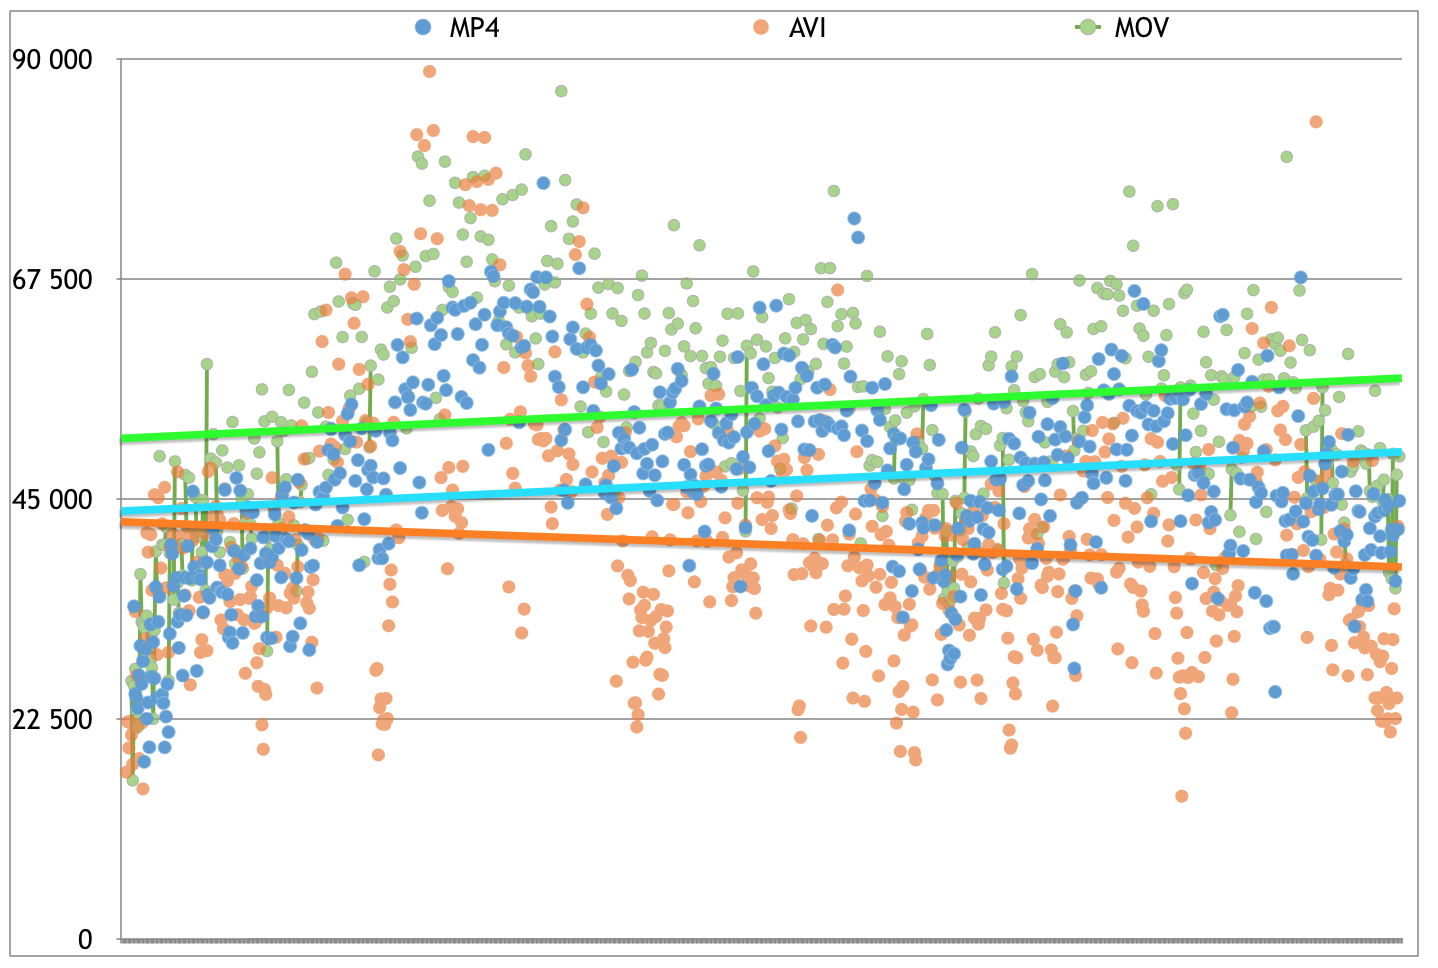
\includegraphics[scale=0.4]{images/codec_performance.png}  
\caption{Performances en fonction du codec}
\end{center}
\end{figure}


\begin{table}[H]
\centering
\caption{Framedrop en fonction du format} 
\bigskip
\begin{tabular}{| l | c | r | }
     \hline
     avi & mp4 & mov \\ \hline
     33\% & 44\% & 52\% \\ \hline
\end{tabular}
\end{table}

On observe que les fichiers les moins compressés (avi) permettent
de meilleures performances. Le poids de la vidéo reste important
mais cela nous semble un sacrifice acceptable. 
L'impact sur les performance des autres formats est non
négligeable, et peut être handicapant sur une petite
configuration. 
\bigskip

Pour la suite de ces test, nous utiliserons les vidéos avi des
clients.

\subsection{Impact des blend}

Pour certaines annotation, nous effectuons des "blend" d'images.
C'est le cas par exemple pour la trace. Cette opération est
coûteuse en ressources (bien plus que de dessiner les
annotations). 
\bigskip

Ici, nous comparons les performances des quatre ordinateurs pour
le traitement d'une vidéo, avec et sans l'utilisation de blend.
Nous lisons simultanément la vidéo avec mouvement de caméra pour
simuler les performances d'une interface avec deux flux vidéo
dont un annoté. 
\bigskip

Le test ici est effectué avec l'éxucatable \textit{test\_time}.



\begin{figure}[H]%
    \centering
    \subfloat[framedrop :
    0\%]{{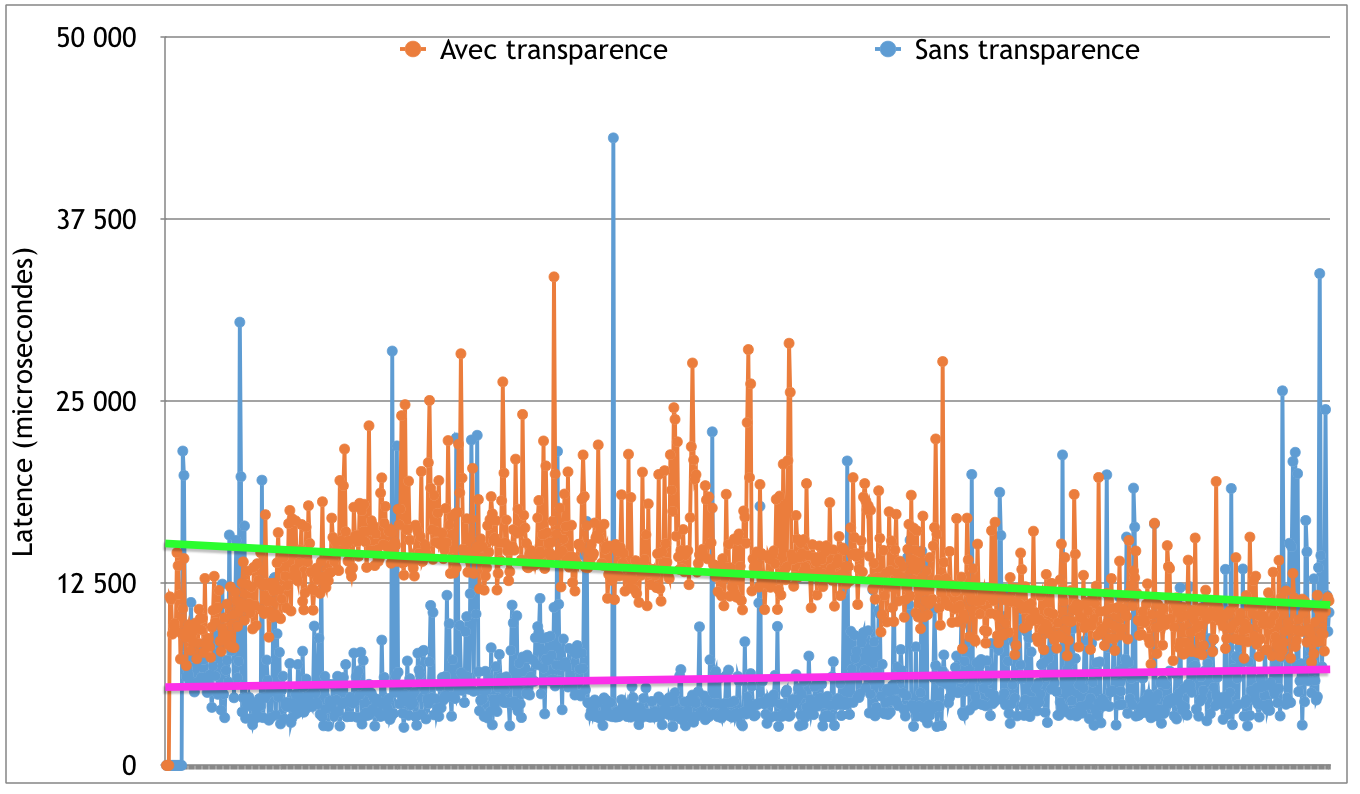
\includegraphics[scale=0.26]{images/time_ouette.png}
    }}%
    \qquad
    \subfloat[framedrop :
    0\%]{{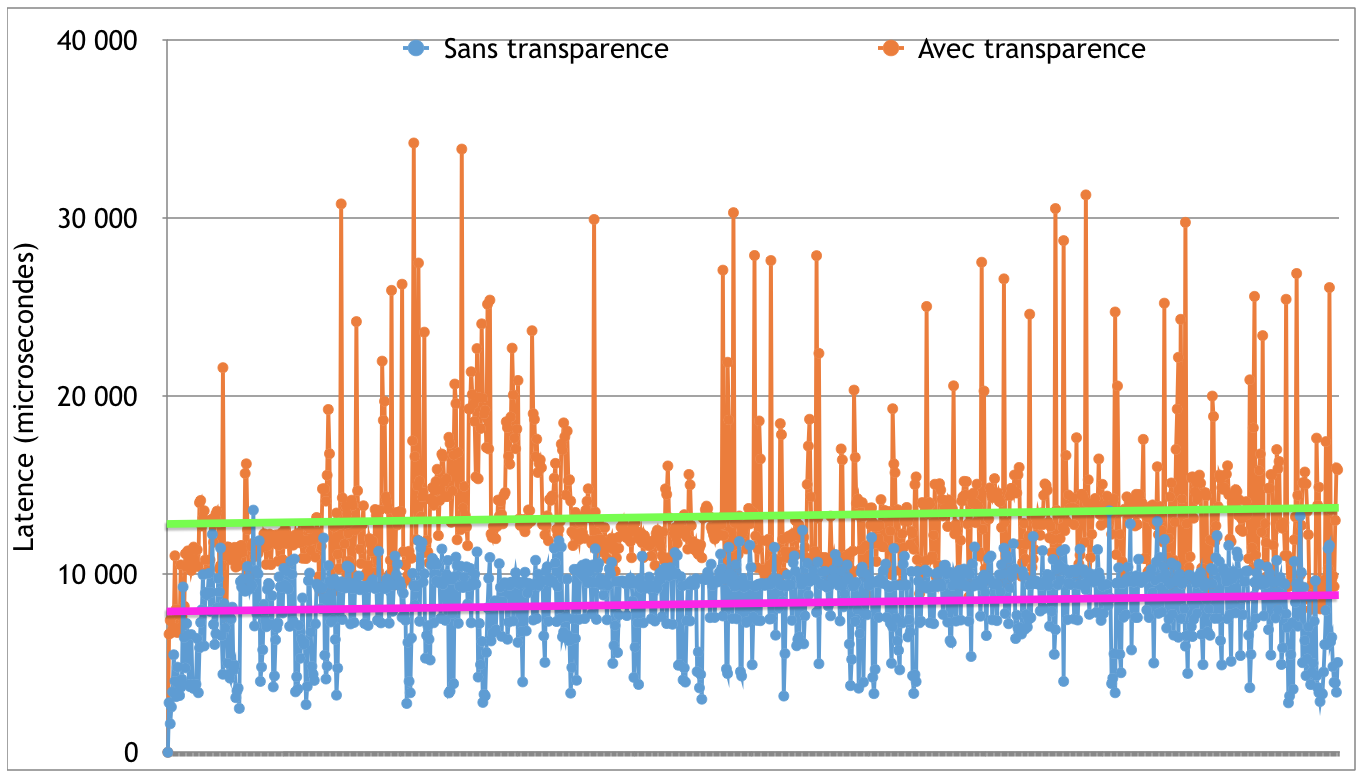
\includegraphics[scale=0.26]{images/time_lulu.png} }}%
    \label{fig:timeAB}%
\end{figure}

\begin{figure}[H]%
    \centering
    \subfloat[framedrop :
    0\%]{{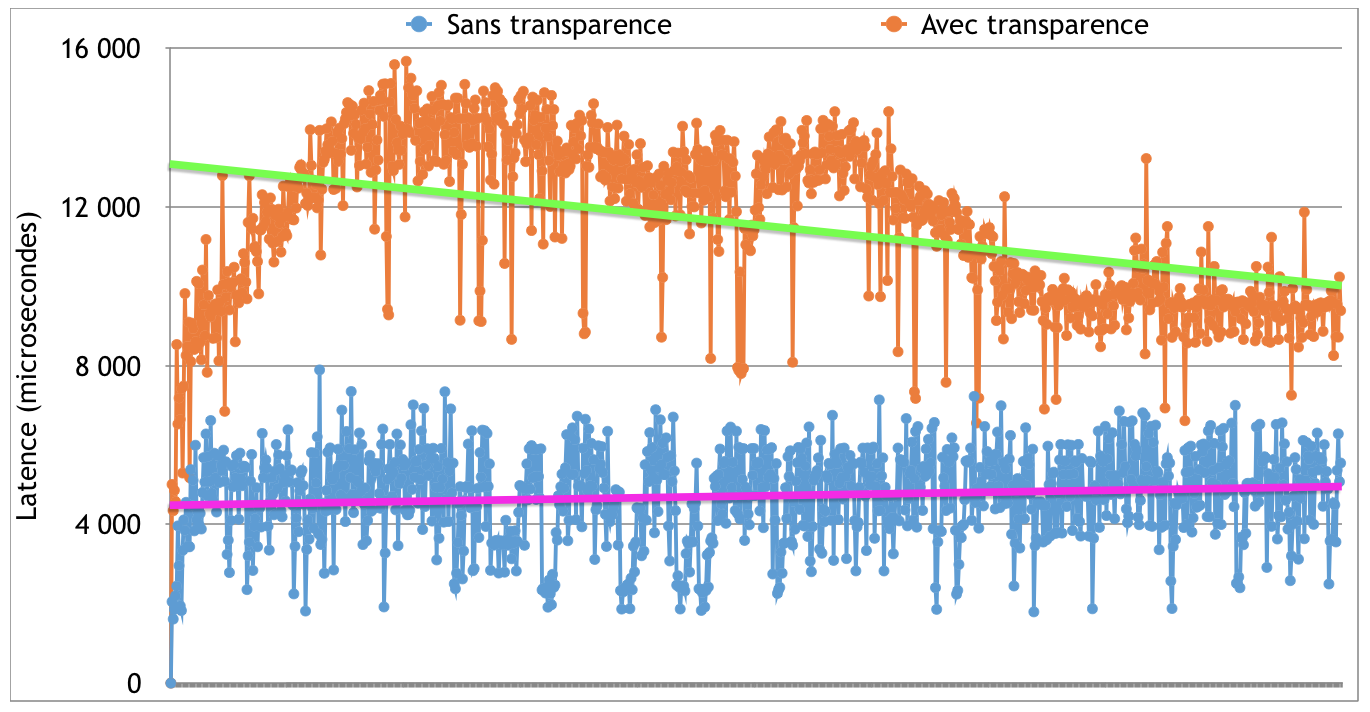
\includegraphics[scale=0.26]{images/time_flo.png} }}%
    \qquad
    \subfloat[framedrop :
    0\%]{{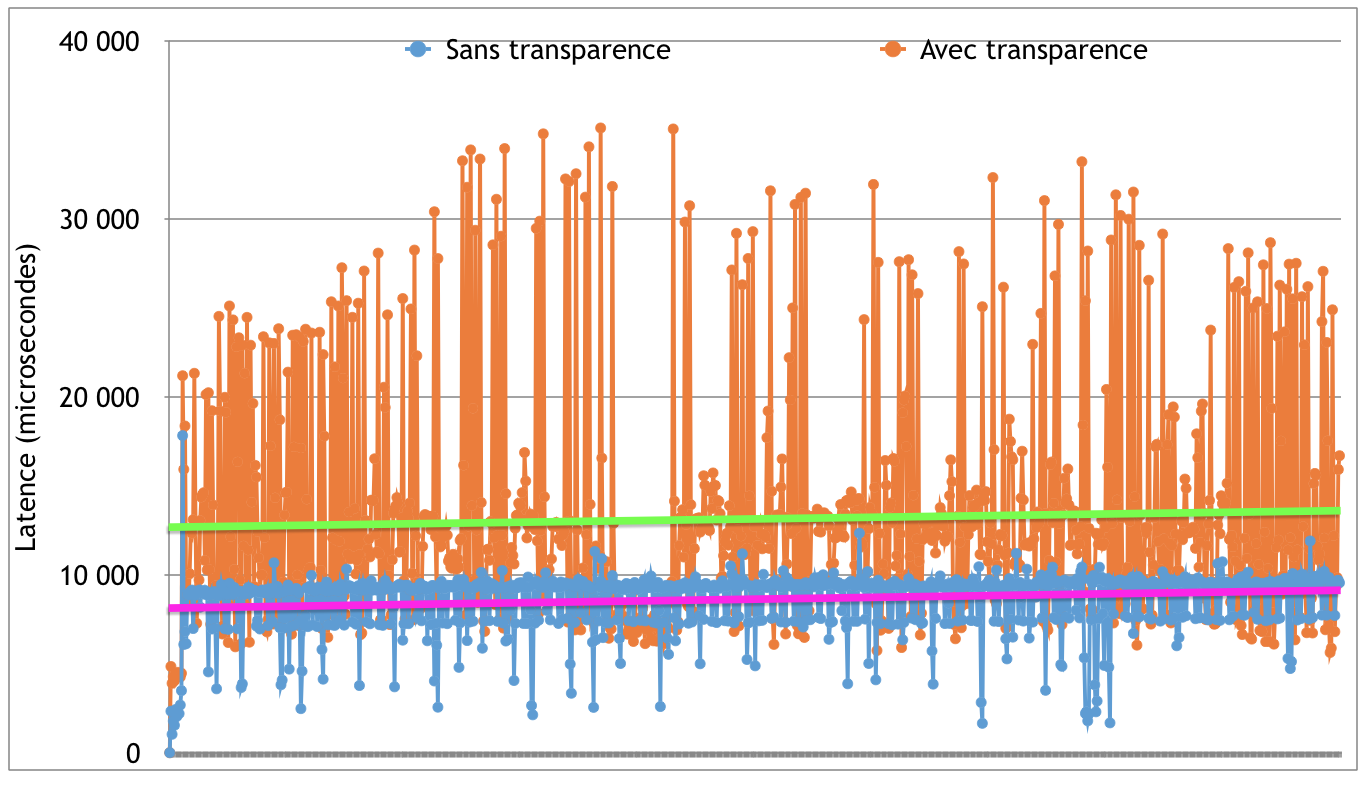
\includegraphics[scale=0.26]{images/time_eliott.png}
    }}%
    \label{fig:timeCD}%
    \caption{Impact du blend sur les performances, deux vidéos}
\end{figure}

\newpage

Nous travaillons ici avec des vidéos 30fps, il faut donc que le
temps de traitement reste inférieure à 33 ms pour éviter les
sauts d'images (ou ralentissements). On observe que tous les
ordinateurs parviennent à rester en dessous de cette limite. En
moyenne, sur les 4 machines, pour deux vidéos simultanées,
l'utilisation de blend augmente le temps de traitement de 80\%. 
\bigskip

Mis à part de rares pics, nous n'observons pas ici de framedrop.
Pour avoir une idée des limites de notre programme dépendamment
de la configuration de la machine, d'autres tests ont été menés. 

\subsection{Limites de puissance}

Ici, nous donnons aux ordinateurs 6 vidéos avec puis sans blend à
traiter simultanément, fichier \textit{test\_video}. Le but est
de déterminer les limites du programme. 
\bigskip

Sur ces graphiques, deux points reliés sont des images qui se
suivent. Dans le cas d'un framedrop, la ligne n'est pas présente.

\begin{figure}[H]%
    \centering
    \subfloat[framedrop :
    50\%]{{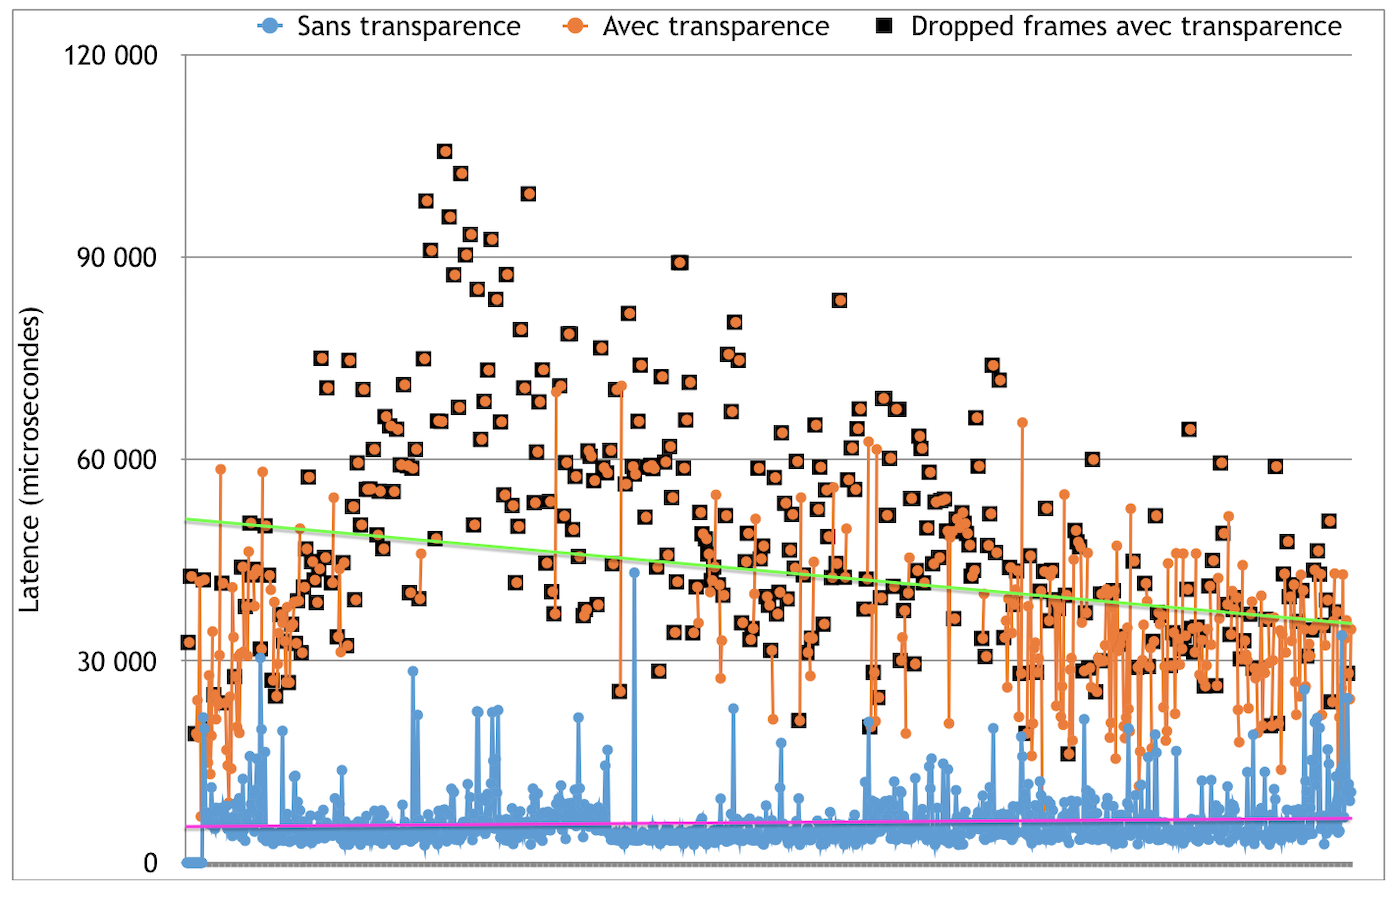
\includegraphics[scale=0.24]{images/video_ouette_50.png} }}%
    \qquad
    \subfloat[framedrop : 47\%
    ]{{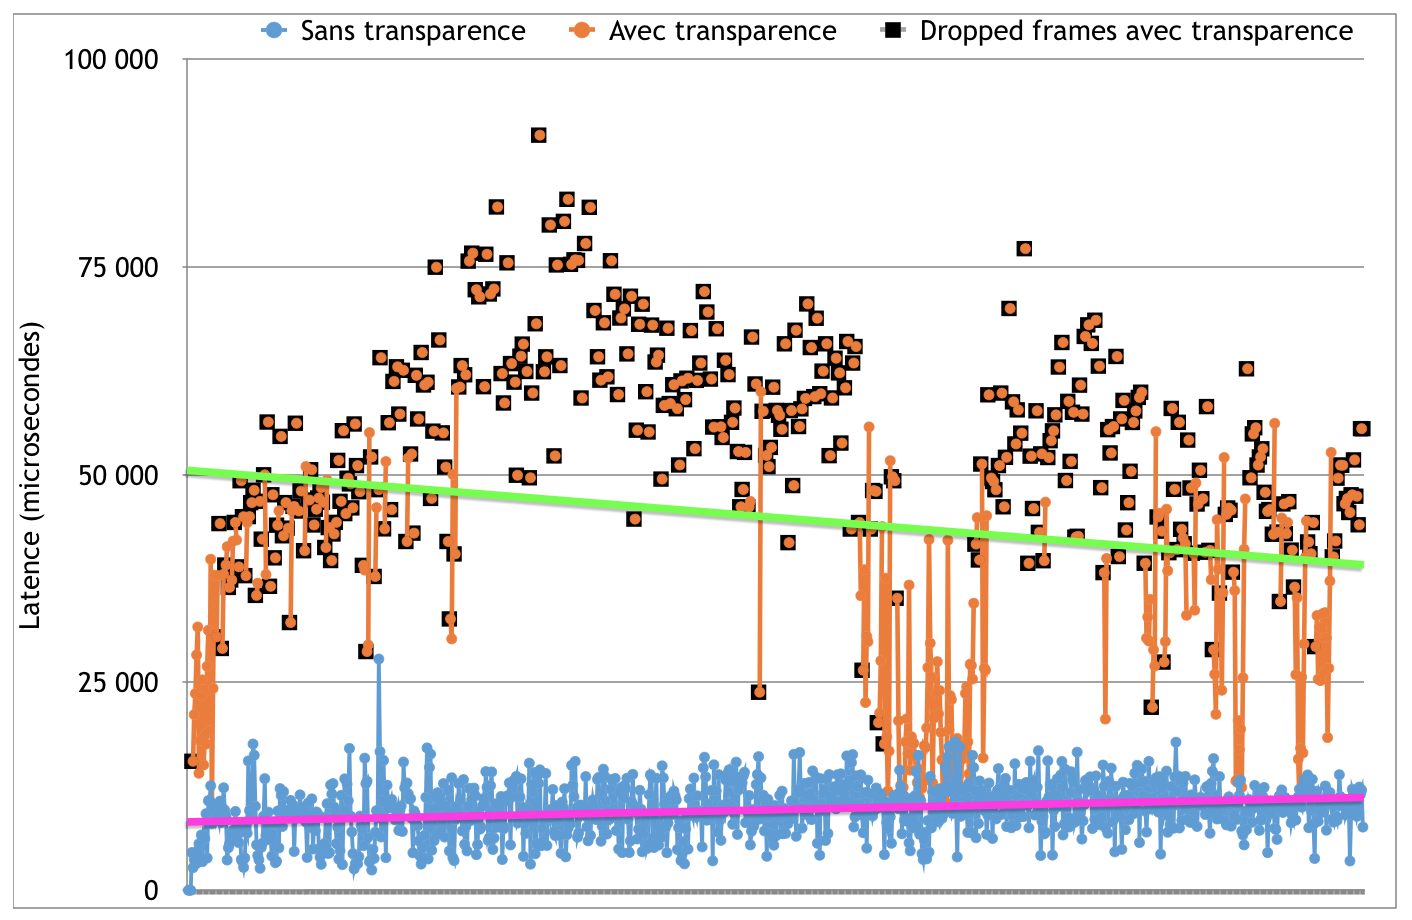
\includegraphics[scale=0.24]{images/video_lulu_47.png} }}%
    \label{fig:videoAB}%
\end{figure}

\begin{figure}[H]%
    \centering
    \subfloat[framedrop :
    17\%)]{{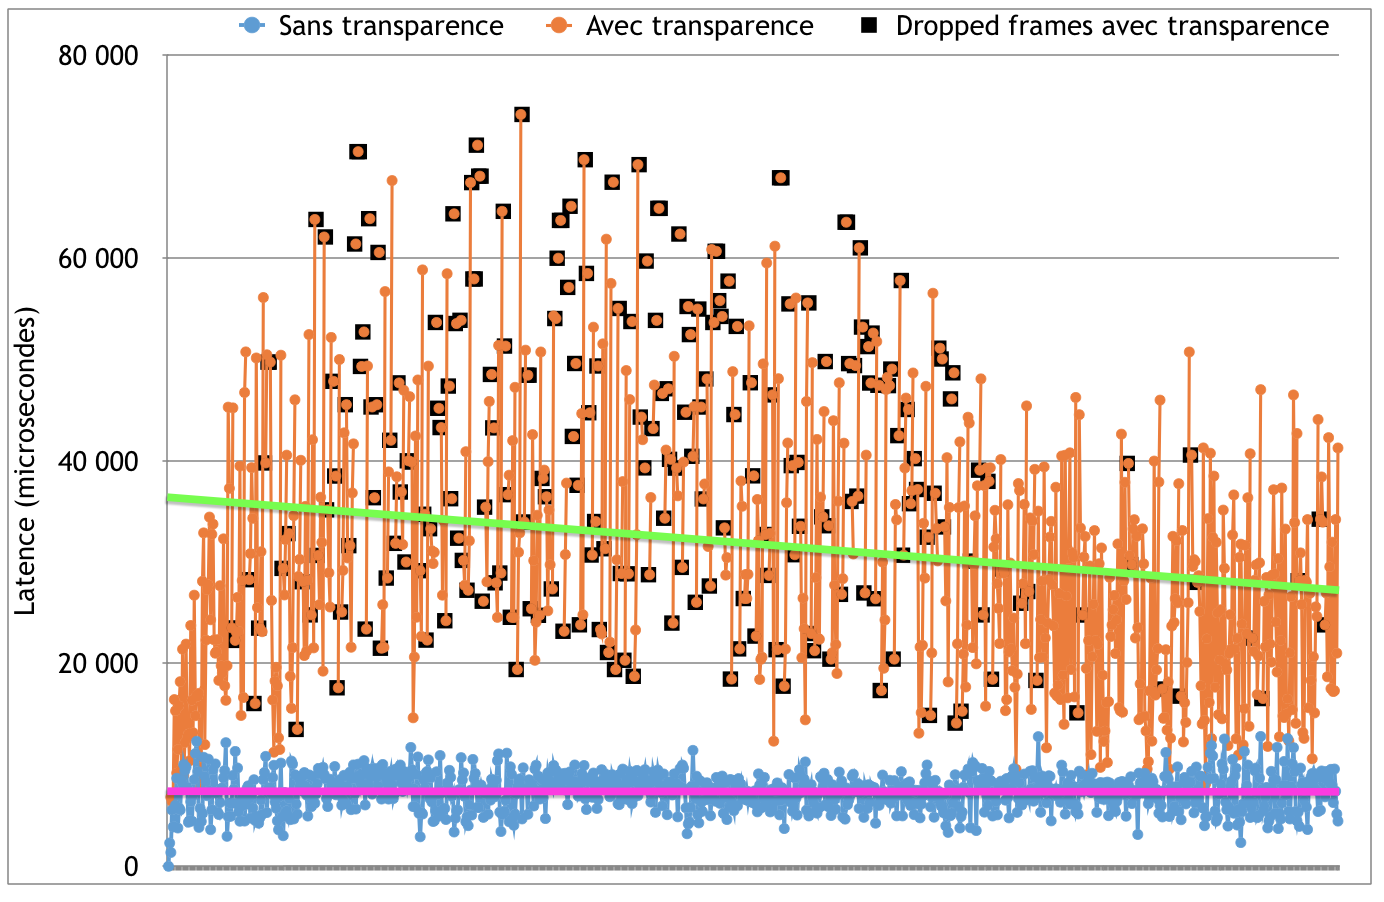
\includegraphics[scale=0.24]{images/video_flo_24.png}
    }}%
    \qquad
    \subfloat[framedrop :
    0\%]{{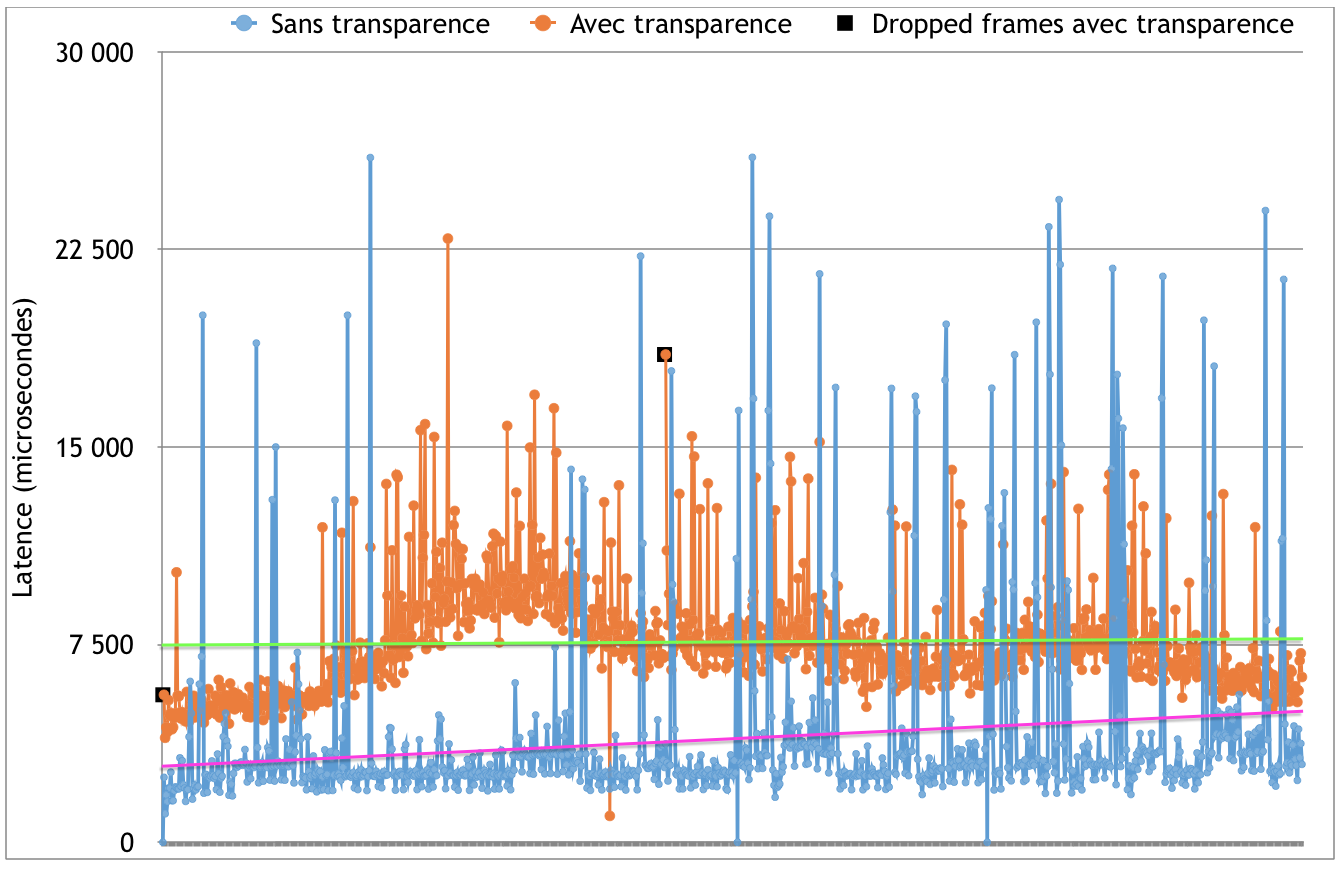
\includegraphics[scale=0.24]{images/video_eliott_0.png}
    }}%
    \label{fig:videoCD}%
    \caption{Limites de puissance}
\end{figure}


Ici nous voyons que les ordinateurs A et B ne parviennent pas à
proposer un traitement en temps réel avec blend sur 6 vidéos à 30
images par secondes de manière fluide. Avec 50\% de frame drop,
la vidéo tombe à environ 15 fps et n'est plus très agréable à
regarder. Les performances de l'ordinateur C sont encore
convenables. L'ordinateur D, contenant les composants les plus
récents, ne semble pas affecté par l'augmentation du nombre de
vidéos.
\bigskip

Pour le traitement des 6 vidéos sans blend, aucun framedrop n'a
eu lieu (à part pics sporadiques).  Les valeurs de latence sont
en moyenne de 4.4ms, très éloignées des 33ms, quand la coupure
s'effectue.
\bigskip

Nous avons continué les expérimentations sur l'ordinateur D pour
déterminer le nombre limite de vidéo qu'il pouvait lire de
manière fluide. 

\begin{figure}[H]  
\begin{center}  
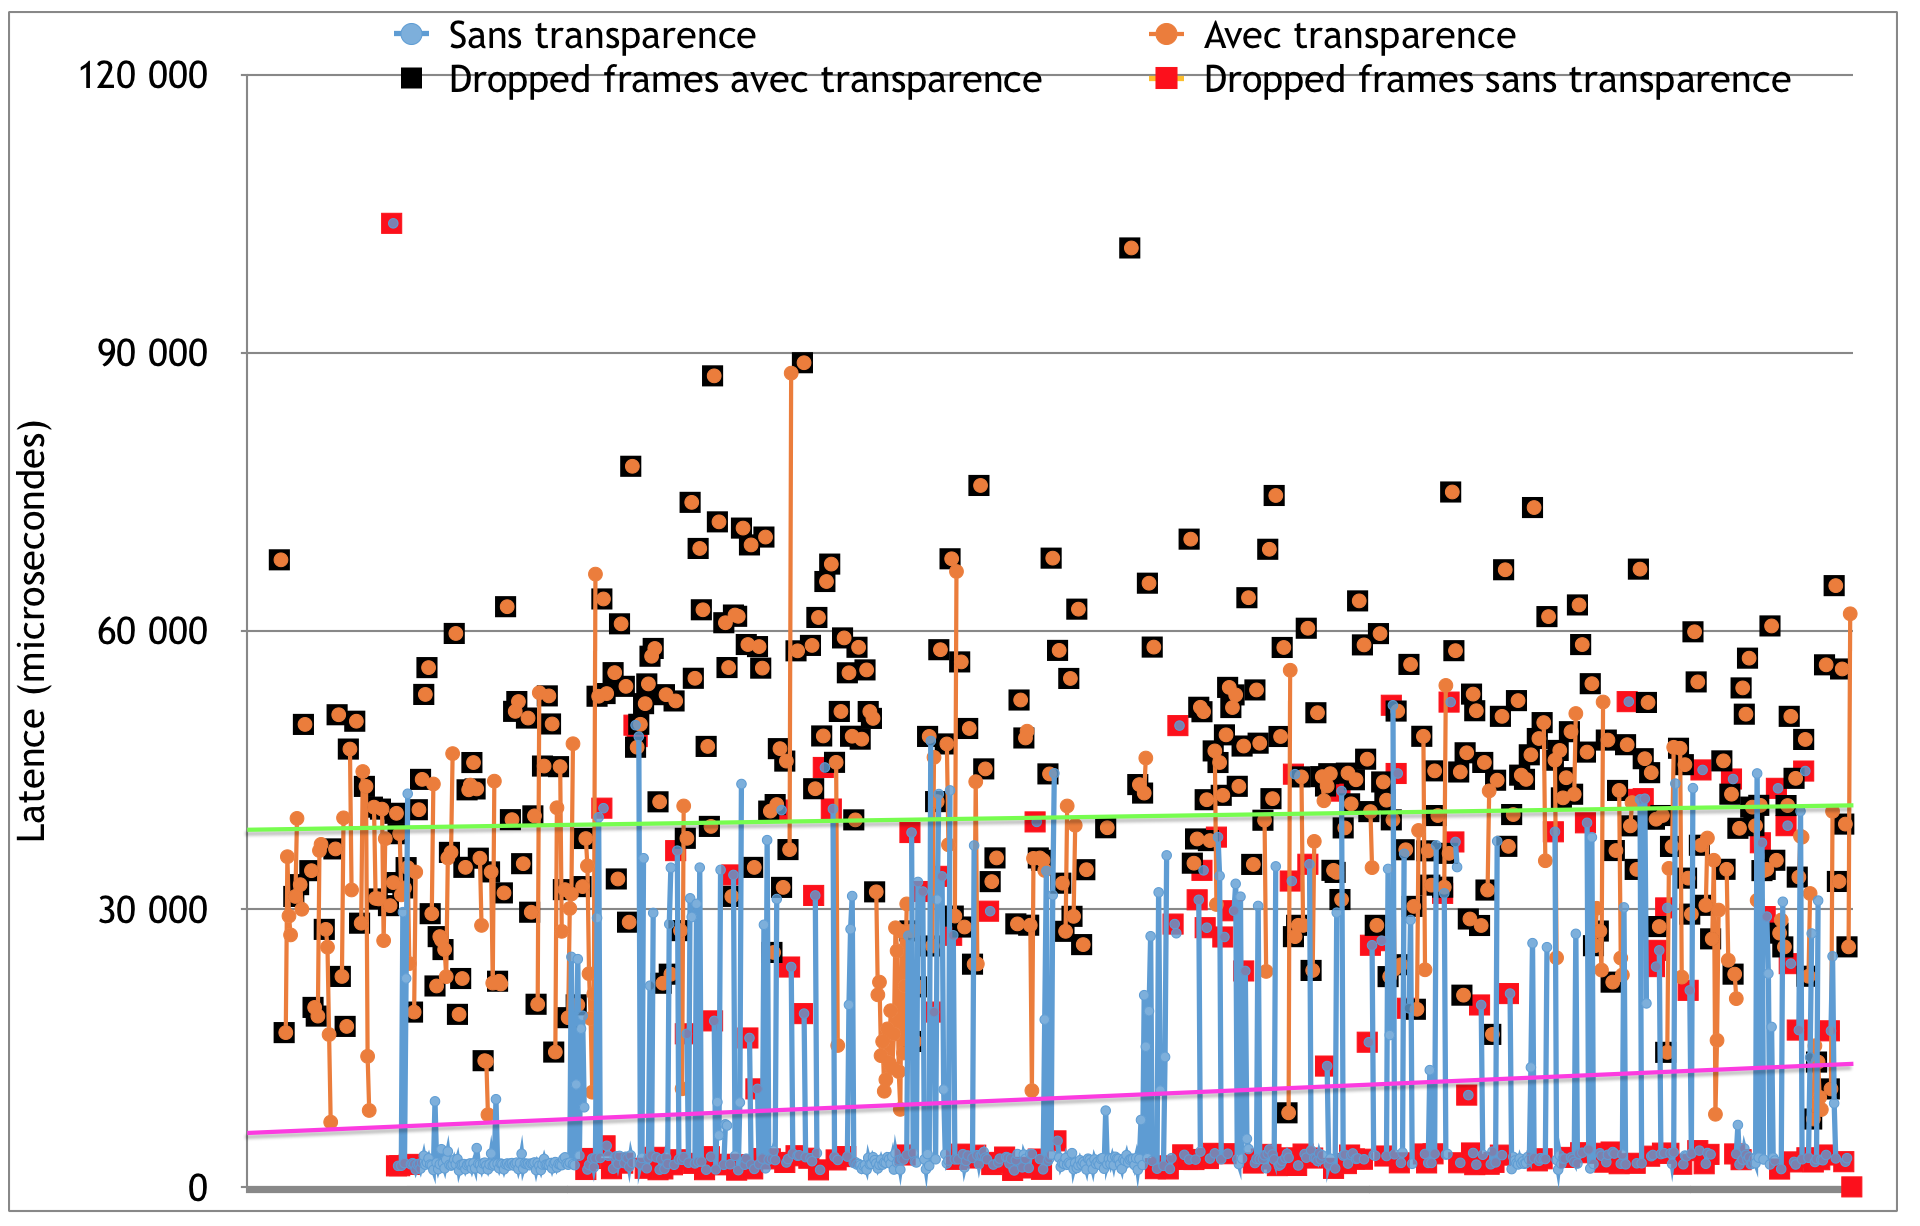
\includegraphics[scale=0.3]{images/video_eliott_20_48_40_37.png} 
\caption{Limites de performances ordinateur D}
\end{center}
\end{figure}

Dans le graphique ci-dessus, nous avons mesuré les performances
de traitement avec blend (transparence) pour 20 vidéos. à partir
de ce nombre, le framedrop devient supérieur à 50\%.
\bigskip

Pour le traitement sans blend, nous avons mesuré sur le même
graphique les performances pour 40 vidéos simultanées. Le
framedrop était de 40\% environ.
\bigskip

L'ordinateur D est celui avec les composants les plus récents
(2017). Ceci semble le favoriser grandement par rapport à
l'ordinateur C, de puissance presque similaire. Si le traitement
ne tourne pas de manière fluide, il faut donc considérer l'achat
de nouveaux composants.
\bigskip

En se basant sur ces résultats et ces proportions de framedrop,
voici performances que l'on peut espérer des ordinateurs avec le
blend : 


\begin{table}[H]
\centering
\caption{Puissance de traitement des ordinateurs (mégapixels/s)} 
\bigskip
\begin{tabular}{| c | c | c | c |}
     \hline
     A & B & C & D \\ \hline
     20 & 35 & 50 & 80 \\ \hline
\end{tabular}
\end{table}


Lors de la rédaction du cahier des besoins, les tests de l'époque
nous faisaient estimer une performance d'environ 80 mégapixels
par seconde sur l'ordinateur C. Ces estimations étaient
pessimistes, et se basaient sur l'incrustation d'une quantité
absurde d'annotation. Le blend toutefois est plus coûteux que le
dessin sur l'image. Ainsi, l'ordinateur C atteint 50 mégapixels/s
avec blend. On a observé un gain de performance d'environ 80\%
sans blend. Ces résultats sont donc cohérents avec nos
prédictions.

